\chapter{Quantum mecahnics in three dimensions}
\section{Schr\"odinger equation in spherical coordinates}
The generalization to three dimsnison is straightforward.
\begin{equation}
  \label{eq:4-1}
  i\hbar \frac{\partial \Psi}{\partial t} = - \frac{\hbar^{2}}{2m} \nabla^{2} \Psi + V\Psi
\end{equation}
where the \textbf{Laplacion} is
\begin{equation}
  \label{eq:4-2}
  \nabla^{2} \equiv \frac{\partial^{2}}{\partial x^{2}} + \frac{\partial^{2}}{\partial y^{2}} + \frac{\partial^{2}}{\partial z^{2}}
\end{equation}
in cartesian coordinates.
With the separation of the variables the general solution gives
\begin{equation}
  \label{eq:4-3}
  \Psi \left( \mathbf{r},t \right) = \sum c_{n} \psi_{n} \left( \mathbf{r} \right) e^{-i E_{n}t/\hbar}.
\end{equation}

\subsection{Separation of variables}
Typically, the potential is a function only of the distance from the origin.
In that case it is natural to adopt \textbf{spehrical coordinates}, as shown in Fig.~\ref{fig:4-1}, the Laplacian takes the form for our time-independent Schr\"odinger equation
\begin{equation}
  \label{eq:4-4}
  \nabla^{2} = \frac{1}{r^{2}} \frac{\partial }{\partial r} \left( r^{2} \frac{\partial}{\partial r} \right) + \frac{1}{r^{2}\sin\theta} \frac{\partial}{\partial \theta} \left( \sin\theta \frac{\partial}{\partial \theta} \right) + \frac{1}{r^{2} \sin^{2} \theta} \left( \frac{\partial^{2}}{\partial \phi^{2}} \right).
\end{equation}
\begin{figure}[h]
  \centering
  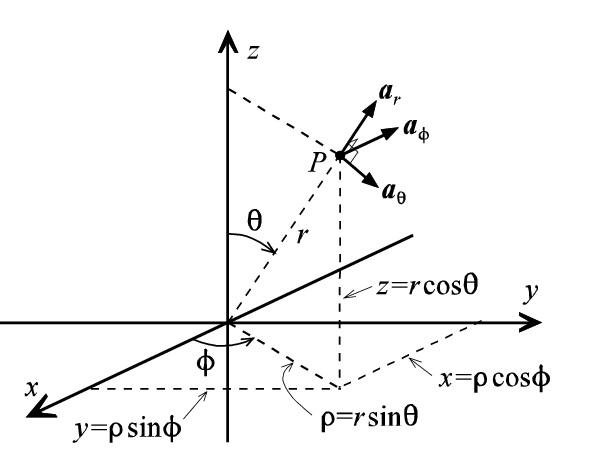
\includegraphics[width=0.45\textwidth]{fig/fig4-1.png}
  \caption{Spherical coordinates.}
  \label{fig:4-1}
\end{figure}

We begin by looking for solutions that are separable into products
\begin{equation}
  \label{eq:4-5}
  \psi \left( r,\theta,\phi \right) = R \left( r \right) Y \left( \theta, \phi \right).
\end{equation}
With this ansatz, we have
\begin{equation}
  \label{eq:4-6}
  \left\{ \frac{1}{R} \frac{\dd}{\dd r} \left( r^{2} \frac{\dd R}{\dd r} \right) - \frac{2mr^{2}}{\hbar^{2}} \left[ V \left( r \right) -E \right] \right\}  + \frac{1}{Y} \left\{  \frac{1}{\sin\theta} \frac{\partial}{\partial \theta} \left( \sin\theta \frac{\partial Y}{\partial \theta} \right) + \frac{1}{ \sin^{2} \theta} \frac{\partial^{2} Y}{\partial \phi^{2}} \right\} = 0
\end{equation}
again each curly bracket should equal to a constant $l \left( l+1 \right)$
\begin{align}
  \label{eq:4-7}
  \left\{ \frac{1}{R} \frac{\dd}{\dd r} \left( r^{2} \frac{\dd R}{\dd r} \right) - \frac{2mr^{2}}{\hbar^{2}} \left[ V \left( r \right) -E \right] \right\} &= l \left( l+1 \right) \\
  \label{eq:4-8}
  \frac{1}{Y} \left\{  \frac{1}{\sin\theta} \frac{\partial}{\partial \theta} \left( \sin\theta \frac{\partial Y}{\partial \theta} \right) + \frac{1}{ \sin^{2} \theta} \frac{\partial^{2} Y}{\partial \phi^{2}} \right\} &= - l \left( l+1 \right).
\end{align}

\subsection{The angular equation}
We first consider Eq.~\eqref{eq:4-8}, which it equals
\begin{equation}
  \label{eq:4-9}
  \sin\theta \frac{\partial}{\partial \theta} \left( \sin\theta \frac{\partial Y}{\partial \theta} \right) + \frac{\partial^{2} Y}{\partial \phi^{2}} = -l \left( l+1 \right) \sin^{2} \theta Y.
\end{equation}
Once again we separate the variables $Y \left( \theta,\phi \right) = \Theta \left( \theta \right) \Phi \left( \phi \right) $.
Equation~\eqref{eq:4-9} can be further separate into two by setting a new constant $m^{2}$
\begin{align}
  \label{eq:4-10}
  \frac{1}{\Theta} \left[ \sin\theta \frac{\dd}{\dd \theta} \left( \sin\theta \frac{\dd \Theta}{\dd \theta} \right) \right] + l \left( l+1 \right) \sin^{2} \theta &= m^{2} \\
  \label{eq:4-11}
  \frac{1}{\Phi} \frac{\dd^{2} \Phi}{\dd \phi^{2}} = - m^{2}
\end{align}
This $\phi$ equation is easy, we have the general solution
\begin{equation}
  \label{eq:4-12}
  \Phi \left( \phi \right) = e^{im\phi}.
\end{equation}
Again we could absorb the canstant into $\Theta$ function.
Since when we rotate $\phi$ by $2\pi$ angle, it back to the same point, it is nature to require that $\Phi \left( \phi + 2\pi \right) = \Phi \left( \phi \right)$.
In other words, we have the constrain such that $\exp \left( 2\pi i m \right)=1$, which means $m$ must be an integer
\begin{equation}
  \label{eq:4-13}
  m = 0, \pm 1, \pm 2, \ldots.
\end{equation}

For the $\theta$ equation in Eq.~\eqref{eq:4-10}, the solution is
\begin{equation}
  \label{eq:4-14}
  \Theta \left( \theta \right) = A P_{l}^{m} \left(\cos \theta \right)
\end{equation}
where $P_{l}^m$ is the \textbf{associated Legendre function}, defined by
\begin{equation}
  \label{eq:4-15}
  P_l^m \left( x \right) \equiv \left( 1-x^2 \right)^{\abs{m}/2} \left( \frac{\dd}{\dd x} \right)^{\abs{m}} P_l \left( x \right) ,
\end{equation}
and $P_l \left( x \right)$ is the $l-$th \textbf{Legendre polynomial}, defined by the \textbf{Rodigures formuale}
\begin{equation}
  \label{eq:4-16}
  P_l \left( x \right) \equiv \frac{1}{2^{l} l!} \left( \frac{\dd}{\dd x} \right)^l \left( x^2 -1 \right)^l.
\end{equation}
Some result of $P_l^m \left( \cos \theta \right)$ is listed in Tab.~\ref{tab:4-1}.
\begin{table}[h]
  \centering
  \begin{tabular}{c c c}
    \toprule
    $P_0^0 = 1$ &  &  \\
    \midrule
    $P_1^0 = \sin \theta$ & $P_1^1= \sin \theta$ & \\
    \midrule
    $P_2^0 = \frac{1}{2} \left( 3 \cos^2 \theta -1 \right)$ & $P_2^1 = 3\sin \theta \cos \theta$ & $P_2^2 = 3 \sin^2\theta$ \\
    \bottomrule
  \end{tabular}
  \caption{Some associated Legendre functions}
  \label{tab:4-1}
\end{table}
Noticee that $l$ must be a nonegation integer because of senseness of the Rodrigues formula in Eq.~\eqref{eq:4-16}.
Moreover, for any $\abs{m}>l$, Eq.~\eqref{eq:4-14} always says $P_l^m=0$.
Then for any given $l$, there are $\left( 2l+1 \right)$ possible value of $m$,\footnote{Notice Eq.~\eqref{eq:4-10} is a second-order differential equation: It should have two linearly independent solutions, for any old values of $l$ and $m$. However the rest of the solution are not physical, because they blow up at $\theta=0, \pi$.}
\begin{equation}
  \label{eq:4-17}
  l = 0, 1, 2, \ldots; ~ ~ m = -l, -l+1, \ldots, -1, 0, 1, \ldots, l-1, l.
\end{equation}

For normalization condition, we have
\begin{equation}
  \label{eq:4-18}
  \int \abs{\psi}^2 r^2 \sin\theta \dd r \dd \theta \dd \phi = \int \abs{R}^2 r^2 \dd r \int \abs{Y}^2 \sin\theta \dd \theta \dd \phi = 1.
\end{equation}
It is convenient to normalize $R$ and $Y$ separately
\begin{equation}
  \label{eq:4-19}
  \int_0^{\infty} \abs{R}^2 r^2 \dd r =1 ~ ~ ~ \text{and} ~ ~ ~ \int_0^{2\pi}\int_0^{\pi} \abs{Y}^2 \sin\theta \dd \theta \dd \phi =1.
\end{equation}
The normalized angular wave functions are called \textbf{spherical harmonics}
\begin{equation}
  \label{eq:4-20}
  Y_l^m \left( \theta,\phi \right) = \epsilon \sqrt{ \frac{\left( 2l+1 \right)}{4\pi} \frac{\left( l-\abs{m} \right)!}{\left( l+\abs{m} \right)!}} e^{im\phi} P_l^m \left( \cos\theta \right),
\end{equation}
where $\epsilon=\left( -1 \right)^{m}$ for $m \geq 0$ and $\epsilon=1$ for $m \leq 0$.
As expected these spherical harmonics function are orthogonal to each other
\begin{equation}
  \label{eq:4-21}
  \int_0^{2\pi} \int_0^{\pi} \left[ Y_l^m \left( \theta,\phi \right) \right]^{*} \left[ Y_{l'}^{m'} \left( \theta,\phi \right) \right] \sin \theta \dd \theta \dd \phi = \delta_{ll'} \delta_{mm'}
\end{equation}
For historical reason, $l$ is called the \textbf{azimuthal quantum number}, and $m$ is the \textbf{magnetic quantum number}.

\subsection{The radial equation}
Notice that the angular part of the wavefunctino, $Y \left( \theta,\phi \right)$, is the same for all spherically symmetric potentials;
The actual shape of the potential affects only the radial part of the wave function, $R \left( r \right)$, which is
\begin{equation}
  \label{eq:4-22}
  \frac{\dd }{\dd r} \left( r^2 \frac{\dd R}{\dd r} \right) - \frac{2mr^{2}}{\hbar^{2}} \left[ V \left( r \right) - E \right] R = l \left( l+1 \right) R.
\end{equation}
One can simplifies this equation if we change the variables
\begin{equation}
  \label{eq:4-23}
  u \left( r \right)  \equiv r R \left( r \right) ,
\end{equation}
and hence we have
\begin{equation}
  \label{eq:4-24}
  - \frac{\hbar^{2}}{2m} \frac{\dd^{2} u}{d r^2} + \left[ V + \frac{\hbar^{2}}{2m} \frac{l \left( l+1 \right)}{r^2} \right] u = Eu.
\end{equation}
This is called the \textbf{radial equation}; it is identical in form to the one-dimentional Schr\"odinger equation Eq.~\eqref{eq:2-5}, except that the \textbf{effective potential},
\begin{equation}
  \label{eq:4-25}
  V_{eff} = V + \frac{\hbar^{2}}{2m} \frac{l \left( l+1 \right)}{r^{2}}.
\end{equation}
Meanwhile the normalization in Eq.~\eqref{eq:4-19} becomes to the form
\begin{equation}
  \label{eq:4-26}
  \int_0^{\infty} \abs{u}^2 \dd r = 1.
\end{equation}
This is as far as we can go before the potential is provoided.

\section{The Hydrogen atom}
The hydrogen atom consists of a heavy motionless proton of charge $e$ together with a light electron that orbits around it.
Forom the Coulomb's law, the potential energy is
\begin{equation}
  \label{eq:4-27}
  V \left( r \right) = - \frac{e^{2}}{4\pi \epsilon_{0}} \frac{1}{r}
\end{equation}
and the radial equation Eq.~\eqref{eq:4-24} reads
\begin{equation}
  \label{eq:4-28}
  - \frac{\hbar^{2}}{2m} \frac{\dd^{2} u}{d r^2} + \left[ - \frac{e^{2}}{4\pi \epsilon_{0}} \frac{1}{r} + \frac{\hbar^{2}}{2m} \frac{l \left( l+1 \right)}{r^2} \right] u = Eu.
\end{equation}
In principle, the Coulomb potential admits continuum sates, (for $ E>0 $ ), describing electron-proton scattering, as wellas discrete bond states, representing the hydrogen atom.
We will focus on the latter case.

\subsection{The radial wave function}
With the new notation\footnote{For bound states, $E$ is negative, so $\kappa$ is real.}
\begin{equation}
  \label{eq:4-29}
  \kappa \equiv \frac{\sqrt{-2mE}}{\hbar},
\end{equation}
then Eq.~\eqref{eq:4-28} reads
\begin{equation}
  \label{eq:4-30}
  \frac{1}{\kappa^{2}} \frac{\dd^{2} u}{\dd r^{2}} = \left[ 1 - \frac{m e^{2}}{2 \pi \epsilon_{0} \hbar^{2} \kappa} \frac{1}{\left(\kappa r\right)} + \frac{l \left( l+1 \right)}{\left( \kappa r \right)^2} \right] u.
\end{equation}
This furter suggests that we have
\begin{equation}
  \label{eq:4-31}
  \rho \equiv \kappa r, ~ ~ ~  \text{and} ~ ~ ~ \rho_0 \equiv \frac{me^{2}}{2\pi \epsilon_{0} \hbar^{2} \kappa},
\end{equation}
so that
\begin{equation}
  \label{eq:4-32}
  \frac{\dd^{2} u}{\dd \rho^{2}} = \left[ 1 - \frac{\rho_{0}}{\rho} + \frac{l \left(l+1\right)}{\rho^{2}} \right] u.
\end{equation}

Let us exame the asymptotic form of the solutions.
As $\rho \to \infty$, the Eq.~\eqref{eq:4-32} can be approximated to
\begin{equation}
  \label{eq:4-33}
  \frac{\dd^{2} u}{\dd \rho^2} = u.
\end{equation}
The general solution is $u \left( \rho \right) = A e^{-\rho} + B e^{\rho}$.
In order to get a finite solution at $\rho \to \infty$, we have to require $B=0$.
So, for large $\rho$ we have
\begin{equation}
  \label{eq:4-34}
  u \left( \rho \right) \sim A e^{-\rho}.
\end{equation}
On the other hand, as $\rho \to 0$ the centrifugal term dominates\footnote{This argument does not apply when $l=0$, although the result we got, Eq.~\eqref{eq:4-36}, is also valid for the case with $l=0$. Here we provides some motivation for Eq. }
\begin{equation}
  \label{eq:4-35}
  \frac{\dd^{2} u}{\dd \rho^{2}} = \frac{l \left( l+1 \right)}{\rho^{2}}  u
\end{equation}
The general solution is $u \left( \rho \right) = C \rho^{l+1} + D \rho^{-l}$.
But we have $D = 0$ since $\rho^{-l}$ blow up as $ \rho \to 0$.
Then the solution is
\begin{equation}
  \label{eq:4-36}
  u \left( \rho \right) \sim C \rho^{l+1}
\end{equation}
for small $\rho$.

The next step is to peel off the asymptotic behavior, introducing a new function $v \left( \rho \right)$
\begin{equation}
  \label{eq:4-37}
  u \left( \rho \right) = \rho^{l+1} e^{-\rho} v \left( \rho \right),
\end{equation}
in the hope that $v \left( \rho \right)$ will turn out to be simpler than $u \left( \rho \right)$.
By calculating $\frac{\dd u}{\dd \rho}$ and $\frac{\dd^{2} u}{\dd \rho^{2}}$, the radial equation, Eq.~\eqref{eq:4-32}, reads
\begin{equation}
  \label{eq:4-38}
  \rho \frac{\dd^{2} v}{\dd \rho^{2}} + 2 \left( l+1 -\rho \right) \frac{\dd v}{\dd \rho} + \left[ \rho_0 - 2 \left( l+1 \right) \right]v =0
\end{equation}
Finally, we assume that $v \left( \rho \right)$ can be expressed as a power series in $\rho$
\begin{equation}
  \label{eq:4-39}
  v \left( \rho \right) = \sum_{j=0}^{\infty} c_j \rho^j.
\end{equation}
Then the problem is boiled down to determine the coefficients.
Differentating term by term, we have
\begin{align*}
  \frac{\dd v}{\dd \rho} &= \sum_{j=0}^{\infty} \left( j+1 \right) c_{j+1} \rho^{j} \\
  \frac{\dd^{2} v}{\dd \rho^2} &= \sum_{j=0}^{\infty} j \left( j+1 \right) c_{j+1} \rho^{j-1}
\end{align*}
Inserting in the Eq.~\eqref{eq:4-38}, we have
\begin{align*}
  &\sum_{j=0}^{\infty} j \left( j+1 \right) c_{j+1} \rho^j + 2 \left( l+1 \right) \sum_{j=0}^{\infty} \left( j+1 \right) c_{j+1} \rho^j \\
  &- 2 \sum_{j=0}^{\infty} j c_j \rho^j + \left[ \rho_0 -2 \left( l+1 \right) \right] \sum_{j=0}^{\infty} c_j\rho^j =0
\end{align*}
Equating the coefficients of the powers yields
\begin{equation}
  \label{eq:4-40}
  c_{j+1} = \left\{ \frac{2 \left(j+l+1\right) - \rho_{0}}{\left(j+1\right) \left(j+2l+2\right)} \right\} c_{j}.
\end{equation}
Form $c_{0}$ whcich is fixed by normalization condition, we can get $c_{j}$.

However, the story is not finished yet!.
For large $j$ (this correspond to large $\rho$, where higher powers dominate), according to Eq.~\eqref{eq:4-40}, we have
\begin{equation*}
  c_{j+1} \cong \frac{2}{j+1} c_{j}.
\end{equation*}
Suppores for a moment that this solution was exact.
Then we have\footnote{That is the reason we keep the term $j+1$.}
\begin{equation}
  \label{eq:4-41}
  c_j= \frac{2^{j}}{j!} c_{0},
\end{equation}
and hence $v \left( \rho \right) = c_0 \sum_{j=0}^{\infty} \frac{2^{j}}{j!} \rho^j = c_0 e^{2\rho}$, whcih result to $u \left( \rho \right) = c_0 \rho^{l+1} e^{\rho}$.
This again blows up at large $\rho$.
To avid this positive exponential, the series must terminate.
There must occur some maximal integer, $j_{max}$, such that
\begin{equation}
  \label{eq:4-42}
  c_{j_{max}+1} = 0.
\end{equation}
This tells us that in Eq.~\eqref{eq:4-40}, we have
\begin{equation*}
  2 \left( j_{max} +l+1 \right) -\rho_0=0.
\end{equation*}
By defining
\begin{equation}
  \label{eq:4-43}
  n \equiv j_{max} + l +1,
\end{equation}
the so-called \textbf{principal quantum number}, we have $\rho_0 = 2n$.
From Eq.~\eqref{eq:4-29} and ~\eqref{eq:4-31}, we know $\rho_0$ is related to the energy $E$.
So the allowed energies are
\begin{equation}
  \label{eq:4-44}
  E_n = - \left[ \frac{m}{2\hbar^{2}} \left( \frac{e^{2}}{4\pi \epsilon_{0}} \right)^2 \right] \frac{1}{n^{2}} = \frac{E_{1}}{n^{2}}, ~ ~ ~ n = 1,2,3,\ldots
\end{equation}
This is the famous \textbf{Bohr formula}.

Considering Eq.~\eqref{eq:4-31}, we have
\begin{equation}
  \label{eq:4-45}
  \kappa = \left( \frac{me^{2}}{4\pi \epsilon_{0} \hbar^{2}} \right) \frac{1}{n} = \frac{1}{an}
\end{equation}
where
\begin{equation}
  \label{eq:4-46}
  a_{0} \equiv \frac{4\pi \epsilon_{0} \hbar^{2}}{m e^{2}} = 0.529 \times 10^{-10} \text{m}
\end{equation}
is the so-called \textbf{Bohr radius}\footnote{Again from Eq.~\eqref{eq:4-31}, we have $\rho = \frac{r}{a_{0} n}$.}.

Now, we can talk about eht spatial wave functions for hydrogen which lateled by three quantum numbers, $n$, $l$, and $m$
\begin{equation}
  \label{eq:4-47}
  \psi_{nlm} \left( r, \theta, \phi \right) = R_{nl} \left( r \right) Y_l^m \left( \theta,\phi \right),
\end{equation}
where from Eq.~\eqref{eq:4-37} and Eq.~\eqref{eq:4-23} we have
\begin{equation}
  \label{eq:4-48}
  R_{nl} \left( r \right) = \frac{1}{r} \rho^{l+1} e^{-\rho} v \left( \rho \right)
\end{equation}
and $v \left( \rho \right)$ is a polynomial of degree $j_{max}= n-l-1$ in $\rho$, whose coefficients are determined by the recursion formula from Eq.~\eqref{eq:4-40} and Eq.~\eqref{eq:4-43},
\begin{equation}
  \label{eq:4-49}
  c_{j+1} = \frac{2 \left( j+l+1-n \right)}{ \left( j+1 \right) \left( j+2l+2 \right)} c_{j} .
\end{equation}

The \textbf{ground state} is in teh case $n=1$; putting in the accepted values for the physical constants, we have
\begin{equation}
  \label{eq:4-50}
  E_1 = - \left[ \frac{m}{2\hbar^{2}} \left( \frac{e^{2}}{4 \pi \epsilon_{0}} \right)^2 \right] = -13.6 ~ \text{eV}.
\end{equation}
So, the \textbf{binding energy} of hydrogen (the amount of energy you would have to impact to the electron in the ground state in order to ionize the atom) is $13.6$ eV.
In ground state, $n=1$, from Eq.~\eqref{eq:4-43} and Eq.~\eqref{eq:4-17} we have
\begin{equation}
  \label{eq:4-51}
  \psi_{100} \left( r,\theta,\phi \right) = R_{10} (r) Y_0^0 \left( \theta,\phi \right).
\end{equation}
Sine $n=1$, we have to force $j_{max}=0$ to get the sensable quantum number in Eq.~\eqref{eq:4-51}.
This, in turn, define the truncate of the recursion formula in Eq.~\eqref{eq:4-49}.
As the result, we have $c_1=0$, so the radical part of the wave function is
\begin{equation}
  \label{eq:4-52}
  R_{10} \left( r \right) = \frac{c_{0}}{a_{0}} e^{- \frac{r}{a_{0}}}
\end{equation}
Normalizaing this the radius part of wavefunction according to Eq.\eqref{eq:4-19}, we have
\begin{equation*}
  \int_0^{\infty} \abs{R_{10}}^{2} r^2 \dd r = 1.
\end{equation*}
So we have $c_0= \frac{2}{\sqrt{a_{0}}}$, and we also have $Y_0^0= \frac{1}{\sqrt{4\pi}}$ from Eq.~\eqref{eq:4-20}.
Then the ground state of hydrogen is
\begin{equation}
  \label{eq:4-53}
  \psi_{100} \left( r,\theta,\phi \right) = \frac{1}{\sqrt{\pi a_{0}^{3}}} e^{- \frac{r}{a_{0}}}.
\end{equation}

For the first excited state, $n=2$, the energy is
\begin{equation}
  \label{eq:4-54}
  E_2 = \frac{-13.6}{2^{2}} ~ \text{eV} = -3.4 ~ \text{eV}.
\end{equation}
Since $n=2$, the posssible quantum numbers are $l=0, m=0$ and $l=1, m=0, \pm 1$, these four different states share this same energy.
If $l=0$, with $n=2$ we know the $j_{max}=1$ and the coefficients are $c_1 = - c_0$ and $c_{2}=0$.
Therefore, we have the radius part of the wavefunction
\begin{equation}
  \label{eq:4-55}
  R_{20} \left( r \right) = \frac{c_{0}}{2a_{0}} \left( 1 - \frac{r}{2a_{0}} \right) e^{- \frac{r}{2a_{0}}} .
\end{equation}
If $l=1$, the recursion formula Eq.~\eqref{eq:4-49} terminate imedinately (since $j_{max}=0$).
Then we have the following result
\begin{equation}
  \label{eq:4-56}
  R_{21} \left( r \right) = \frac{c_{0}}{4 a_{0}^{2}} r e^{- \frac{r}{2a_{0}}} .
\end{equation}

More general, for arbitrary $n$, the possible values of $l$ from Eq.~\eqref{eq:4-43} are
\begin{equation}
  \label{eq:4-57}
  l = 0,1,2,\ldots, n-1,
\end{equation}
and for each $l$ from Eq.~\eqref{eq:4-17} there are $\left( 2l+1 \right)$ possible values of $m$.
Then the total degeneracy of the energy level $E_n$ is
\begin{equation}
  \label{eq:4-58}
  d \left( n \right) = \sum_{l=0}^{n-1} \left( 2l+1 \right) = n^{2}.
\end{equation}
The polynomial $v \left( \rho \right)$ defined in Eq.~\eqref{eq:4-39} and Eq.~\eqref{eq:4-49} is a well known functiion
\begin{equation}
  \label{eq:4-59}
  v \left( \rho \right) = L_{n-l-1}^{2l+1} \left( 2\rho \right)
\end{equation}
where
\begin{equation}
  \label{eq:4-60}
  L_{q-p}^p \left( x \right) \equiv \left( -1 \right)^p \left( \frac{\dd}{\dd x} \right)^p L_q lr(x)
\end{equation}
is the \textbf{associated Laguerre polynomial}, and
\begin{equation}
  \label{eq:4-61}
  L_q \left( x \right) \equiv e^x \left( \frac{\dd }{\dd x} \right)^q \left( e^{-x} x^q \right)
\end{equation}
is the $q$th \textbf{Laguerre polynomial}.
The normalized hydrogen wave function are
\begin{equation}
  \label{eq:4-62}
  \psi_{nlm} = \sqrt{ \left(\frac{2}{n a_{0}}\right)^{3} \frac{\left(n-l-1\right)!}{2n \left[\left(n+l\right)!\right]^3} } e^{- \frac{r}{n a_{0}}} \left( \frac{2r}{n a_{0}} \right)^l \left[ L_{n-l-1}^{2l+1} \left( \frac{2r}{na_{0}} \right) \right] Y_l^m \left( \theta,\phi \right)
\end{equation}
The density plots are shown in Fig.~\ref{fig:4-2}.
\begin{figure}[h]
  \centering
  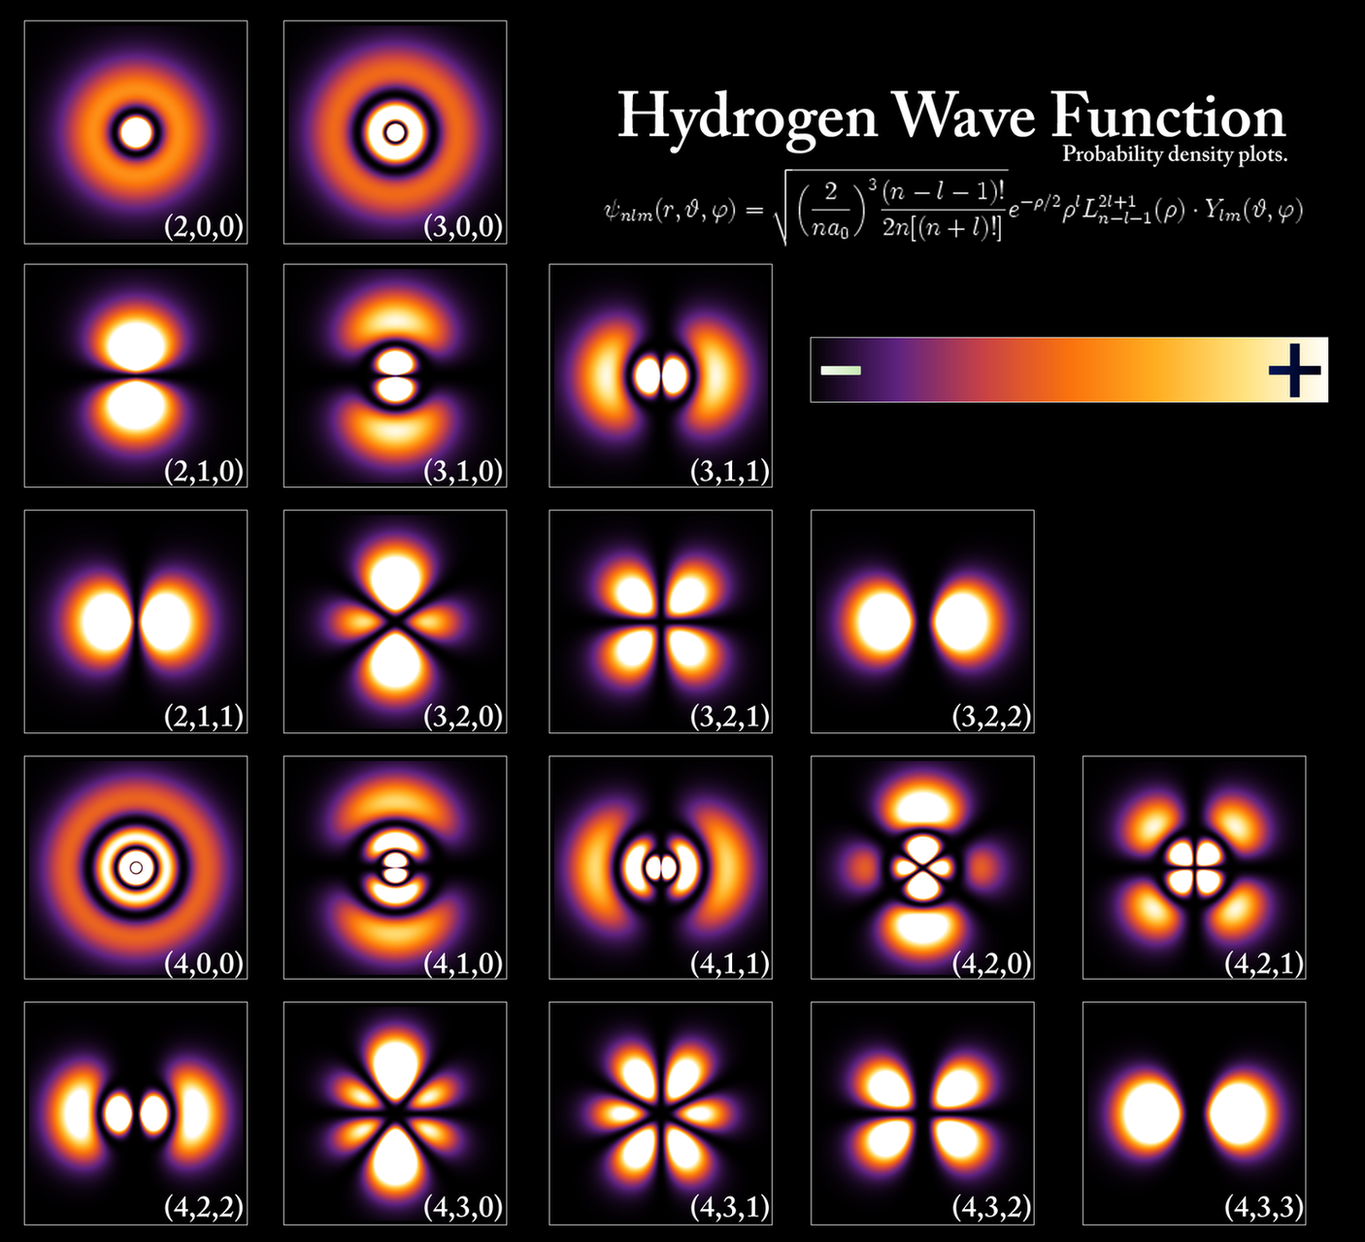
\includegraphics[width=1.\textwidth]{fig/fig4-2.png}
  \caption{Density plot of the wavefunction $\abs{\psi}^2$ for different quantum number.}
  \label{fig:4-2}
\end{figure}

Notice that the wave functions depend on all three quantum numbers, the energy in Eq.~\eqref{eq:4-44} are determined by $n$ alone.
This is a peculiarity of the Coulomb poential\footnote{For the case of infinity spherical well, the energy depend also on $l$.}.
The wave function are mutually orthogonal inherit from the spherical harmonic function in Eq.~\eqref{eq:4-21}
\begin{equation}
  \label{eq:4-63}
  \int \psi^{*}_{nlm} \psi_{n'l'm'} r^2 \sin \theta \dd  \dd \theta \dd \phi = \delta_{nn'} \delta_{ll'} \delta_{mm'},
\end{equation}
where $\delta_{n n'}$ is from the fact that they are eigenfunction of different eigenvalues from the Hamiltonian.

\subsection{The spectrum of Hydrogen}
In principle, if you put a hydrogen atom into some station state $\Psi_{nlm}$, is should stay there forever.
However if you tickle it silghtly (by collision with other atom, or by shining light on it), the electron may undergo a \textbf{transition} to some other station state --- either by absorbing energy and moving up to a higher-energy state, or by giving off energy and moving down.
In practice such perturbations are always present; transitions are constantly occurring, and the result is that a container of hydrogen gives off phonons, whose energy corresponds to the difference in energy between the initial and final states
\begin{equation}
  \label{eq:4-64}
  E_{\gamma} = E_i-E_f = -13.6 \left( \frac{1}{n_{i}^2} - \frac{1}{n_{f}^{2}} \right) .
\end{equation}

According to \textbf{Planck formula}, the energy of a photon is proportional to its frequency
\begin{equation}
  \label{eq:4-65}
  E_{\gamma}  = h \nu
\end{equation}
Meanwhile, the wavelength is given by $\lambda = \frac{c}{\nu}$, so
\begin{equation}
  \label{eq:4-66}
  \frac{1}{\lambda}= R \left( \frac{1}{n_{f}^{2}} - \frac{1}{n_{i}^{2}} \right)
\end{equation}
where
\begin{equation}
  \label{eq:4-67}
  R \equiv \frac{m}{4\pi c \hbar^{2}}  \left( \frac{e^{2}}{4 \pi \epsilon_{0}} \right)^2 = 1.097 \times 10^7 \text{m}^{-1}
\end{equation}
is known as the \textbf{Rydberg constant}.
Equation ~\eqref{eq:4-66} is the \textbf{Rydberg formula} for the spectrum of hydrogen.
This is discovered empiically in the nineteenth centry, and it was Bohr's theory to explain the result and calculate $R$ in terms of the fundamental constants of nature.

\section{Angular momentum}
For stationary state, the hydrogen atom are labeled by three quantum numbers: the principal quantum number, $n$, determines the energy of the state; for $l$ and $m$ are related to the orbital angular momentum.
In classical theory of central forces, energy and angular momentum are the fundamental conserved quantities, and it it not supersing that angular momentum plays a significant role in the quantum theory.

Classically, the angular momentum of a particle is given by
\begin{equation}
  \label{eq:4-68}
  \mathbf{L}  = \br \times \bp.
\end{equation}
The corresponding quantum operaors are obtained by the standard prescrition with $p_x \to - i\hbar \frac{\partial}{\partial x}$ and so on.

\subsection{Eigenvalues}
First the operators are not commute with each other
\begin{equation}
  \label{eq:4-69}
  \left[ L_x, L_y \right] = i\hbar L_{z} .
\end{equation}
We could cycly permutate the subindices to get the similar result for other directions.
They are the fundamantal commutation relations for angular momentum

Notice that $L_x$, $L_y$, and $L_z$ are \textit{incompatible} observables, the generalized uncertainty principle indicates that $\sigma_{L_x} \sigma_{L_y} \geq \frac{\hbar}{2} \abs{\expval{L_{z}}}$.
It would therefore be futile to look for states that are simultaneously eigenfunctions of $L_x$ and $L_y$.
On the other hand, the \textit{square of the total angular momentum}
\begin{equation}
  \label{eq:4-70}
  L^2 \equiv L_x^2 + L_y^2 + L_z^2
\end{equation}
does commute with $L_{i=x,y,z}$
\begin{equation}
  \label{eq:4-71}
  \left[ L^2, L_{i=x,y,z} \right] =0.
\end{equation}
or, in a more compact way\footnote{To prove the relation, we use the follow identity $\left[ AB,C \right] = A \left[ B,C \right] + \left[ A,C \right]B$.}
\begin{equation}
  \label{eq:4-72}
  \left[ L^2, \bL \right] =0.
\end{equation}
So $L^2$ is compatible with each component of $\bL$, and we can hope to find simultaneous eigenstates of $L^2$ and $L_z$ for example,
\begin{equation}
  \label{eq:4-73}
  L^2 f = \lambda f ~ ~ ~ \text{and} ~ ~ ~ L_z f = \mu f.
\end{equation}

Using the ladder operator technique
\begin{equation}
  \label{eq:4-74}
  L_{\pm} \equiv L_x \pm i L_{y}.
\end{equation}
The commutator with $L_z$ and $L^{2}$ are
\begin{align}
  \label{eq:4-75}
  \left[ L_z, L_{\pm} \right] &= \pm \hbar L_{\pm}, \\
  \label{eq:4-76}
  \left[ L^2, L_{\pm} \right] &=0.
\end{align}
With Eq.~\eqref{eq:4-76}, we know that if $f$ is an eigenfunction of $L^2$ and $L_z$, so also is $L_{\pm}f$.
With Eq.~\eqref{eq:4-75} and Eq.~\eqref{eq:4-73}, we have
\begin{equation}
  \label{eq:4-77}
  L_z \left( L_{\pm} f \right) = \left( L_z L_{\pm} - L_{\pm} L_z \right) f + L_{\pm} L_z f = \pm \hbar L_{\pm} f + L_{\pm} \left( \mu f \right) = \left( \mu \pm \hbar \right) \left( L_{\pm} f \right),
\end{equation}
so $L_{\pm} f$ is an eigenfunction of $L_z$ with the \textit{new} eigenvalue $\mu \pm \hbar$.

For a given value of $\lambda$, we obtain a ladder of states, with each rung spearated form its neighbors by one unit of $\hbar$ in the eigenvalue of $L_z$.
This ladder is not infinit long, one can not reach a state for which the $z$-component exceeds the total\footnote{Formally, we have $\expval{L^{2}} = \expval{L_x^2} + \expval{L_y^2} + \expval{L_z^2}$, but we also have $\expval{L_x^2} = \braket{L_x f} \geq 0$ for $x$- and $y$-direction. Then $\lambda = \expval{L_x^2} + \expval{L_y^2} + \mu^2 \geq \mu^{2}$.}.
There must exit a ``top rung'', $f_t$, such that\footnote{Actually all we can conclude is that $L_+f_t$ is not normalizable. Check the problem.}
\begin{equation}
  \label{eq:4-78}
  L_+f_t =0.
\end{equation}

Let $\hbar l$ be the eigenvalue of $L_z$ at this top rung,
\begin{equation}
  \label{eq:4-79}
  L_zf_t =\hbar l f_t; ~ ~ ~ L^2 f_t = \lambda f_t
\end{equation}
Now, with the identity
\begin{equation}
  \label{eq:4-80}
  L^2 = L_{\pm} L_{\mp} + L_z^2 \mp \hbar L_{z}
\end{equation}
we can calculate the eigenvalue
\begin{equation*}
  L^2 f_t = \left( L_- L_+ + L_z^2 + \hbar L_z \right) f_t = \left( 0 + \hbar^2l^2 +\hbar^2 l \right) f_t = \hbar^2 l \left( l+1 \right) f_t
\end{equation*}
and hence
\begin{equation}
  \label{eq:4-81}
  \lambda = \hbar^2 l \left( l+1 \right).
\end{equation}
This tell us the eigenvalue of $L^2$ in terms of the \textit{maximum eigenvalue} of $L_z$.

Meanwhile, there is also a ``bottom rung'', $f_b$, such that $L_- f_b = 0$.
Let $\hbar \bar{l}$ be the eigenvalue of $L_z$ at this bottom rung $L_z f_b = \hbar \bar{l}f_{b}$.
Using Eq.~\eqref{eq:4-80}, we have
\begin{equation}
  \label{eq:4-82}
  \lambda = \hbar^2 \bar{l} \left( \bar{l} - 1 \right).
\end{equation}
Comparing Eq.~\eqref{eq:4-81} and Eq.~\eqref{eq:4-82}, we see that $l \left( l+1 \right) = \bar{l} \left( \bar{l}-1 \right)$, so either $\bar{l} = l+1$ (which is absurd, the bottom rung is higher than the top rung) or else
\begin{equation}
  \label{eq:4-83}
  \bar{l} = -l.
\end{equation}

Appearently, from Eq.~\eqref{eq:4-83}, we known the eigenvalue of $L_z$ are $m\hbar$ where $m$ goes form $-l$ to $+l$ in $N$ integer steps.
In particular, it follows that $l=-l +N$, and hence $l= \frac{N}{2}$, so $l$ \textit{must be an integer or a half-integer}.
Then the eigenfunctions are characterized by the number $l$ and $m$
\begin{equation}
  \label{eq:4-84}
  L^2 f_l^m = \hbar^2 l \left( l+1 \right) f_l^m; ~ ~ ~ L_zf_l^m = \hbar m f_l^m
\end{equation}
where
\begin{equation}
  \label{eq:4-85}
  l = 0, \frac{1}{2}, 1, \frac{3}{2}, \ldots ; ~ ~ ~  m = -l, -l+1, \ldots, l-1, l.
\end{equation}
For a given value $l$, there are $2l+1$ different values of $m$.

Usually, peopel like to illustrate this result with the diagram Fig.~\ref{fig:4-3}.
\begin{figure}[h]
  \centering
  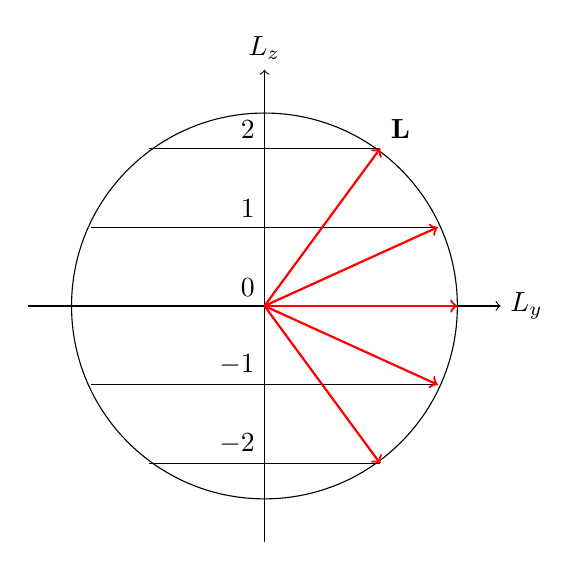
\begin{tikzpicture}
    \draw [->] (0,-3) -- (0,3);
    \draw [->] (-3,0) -- (3,0);
    \draw (0,0) circle [radius=2.45];
    \draw (-1.47,2) -- (1.47,2);
    \draw (-2.2,1) -- (2.2,1);
    \draw (-1.47,-2) -- (1.47,-2);
    \draw (-2.2,-1) -- (2.2,-1);
    \draw [thick, red, ->] (0,0) -- (1.47,2);
    \draw [thick, red, ->] (0,0) -- (2.2,1);
    \draw [thick, red, ->] (0,0) -- (2.45,0);
    \draw [thick, red, ->] (0,0) -- (1.47,-2);
    \draw [thick, red, ->] (0,0) -- (2.2,-1);
    \node [above left] at (0,2)  {$2$};
    \node [above left] at (0,1)  {$1$};
    \node [above left] at (0,0)  {$0$};
    \node [above left] at (0,-1)  {$-1$};
    \node [above left] at (0,-2) {$-2$};
    \node [above] at (0,3) {$L_z$};
    \node [right] at (3,0) {$L_y$};
    \node [above right] at (1.48, 2) {$\mathbf{L}$};
  \end{tikzpicture}
  \caption{Angular momentum startes for $l=2$.}
  \label{fig:4-3}
\end{figure}
The red arrows are supposed to represent possible angular momenta --- in units of $\hbar$ where they all have same length $\sqrt{l \left( l+1 \right)}$ and their $z$ components are allowed values of $m=-2,-1,0,1,2$.
Notice that the magnitude of the vectors is greater than the maximum $z$ component\footnote{In general, $\sqrt{l \left( l+1 \right)} > l$, except for the ``trival'' case $l=0$.}.
Evidently, you can not get the angular momentum to point perfectly along the $z$ direction.
Since to do this, you have to know all thee components simutaneously($L_x=L_y=0, L_z = \sqrt{l \left( l+1 \right)}$), and the uncertainty priciple tell us that is impossible.
It is not merely that you don't know all three components of $\mathbf{L}$; there simply aren't three components---a particle just cannot have a determinate angular momentum vector, any moer than it can simultaneously have a determinate position and moemntum.
If $L_z$ has a well-defined value, the $L_x$ and $L_y$ do not.

So, by purely algebraic means, starting with the fundamental commutation relations for angular momentum Eq.~\eqref{eq:4-69}, we have determined the eigenvalues of $L^2$ and $L_z$---without ever seeing the eigenfunctions themselves!
For the eigenfunctions, $f_l^m=Y_l^m$---the eigenfunctions of $L^2$ and $L_z$ are noting but the old sperical harmoincs function in Eq.~\eqref{eq:4-20}.
Since they are eigenfunctions of hermitian operators, $L^2$ and $L_z$, belonging to distinct eigenvalues.

\subsection{Eigenfunctions}
First, we rewrite the angular momentum in sperical coordinates, since $\mathbf{L} = \frac{\hbar}{i} \left( \mathbf{r} \times \nabla \right)$, and the gradient
\begin{equation}
  \label{eq:4-86}
  \nabla = \hat{r} \frac{\partial}{\partial r} + \hat{\theta} \frac{1}{r} \frac{\partial}{\partial \theta} + \hat{\phi} \frac{1}{r\sin\theta} \frac{\partial}{\partial \phi}
\end{equation}
meanwhile, $\mathbf{r}= r \hat{r}$, so
\begin{equation}
  \label{eq:4-87}
  \mathbf{L} = \frac{\hbar}{i} \left( \hat{\phi} \frac{\partial}{\partial \theta} - \hat{\theta} \frac{1}{\sin \theta} \frac{\partial}{\partial \phi} \right) .
\end{equation}
The unit vectors $\hat{\theta}$ and $\hat{\phi}$ can be resolved into their cartesian components due to Fig.~\ref{fig:4-1}
\begin{align}
  \label{eq:4-88}
  \hat{\theta} &= \left( \cos\theta \cos\phi \right) \hat{x} + \left( \cos\theta \sin\phi \right) \hat{y} - \left( \sin\theta \right) \hat{z} \\
  \label{eq:4-49}
  \hat{\phi} &= -\left( \sin\phi \right) \hat{x} + lr(\cos\phi) \hat{y}
\end{align}
Thus we have
\begin{align}
  \label{eq:4-90}
  L_x &= \frac{\hbar}{i} \left( -\sin\phi \frac{\partial}{\partial \theta} - \cos\phi \cot \theta \frac{\partial}{\partial \phi} \right),\\
  \label{eq:4-91}
  L_y &= \frac{\hbar}{i} \left( +\cos\phi \frac{\partial}{\partial \theta} - \sin\phi \cot \theta \frac{\partial}{\partial \phi} \right),\\
  \label{eq:4-92}
  L_z &= \frac{\hbar}{i} \frac{\partial}{\partial \phi}.
\end{align}
For descending and increasing operators
\begin{equation}
  \label{eq:4-93}
  L_{\pm} = \pm \hbar e^{\pm \phi} \left( \frac{\partial}{\partial \theta} \pm i \cot \theta \frac{\partial}{\partial \phi} \right).
\end{equation}
and $L^2$,
\begin{equation}
  \label{eq:4-94}
  L^2 = -\hbar^2 \left[ \frac{1}{\sin\theta} \frac{\partial}{\partial \theta} \left( \sin\theta \frac{\partial}{\partial \theta} \right) + \frac{1}{\sin^{2} \theta} \frac{\partial^{2}}{\partial \phi^{2}} \right] .
\end{equation}

We are now in a position to determine $f_l^m \left( \theta,\phi \right)$.
It's an eigenfunction of $L^2$, with eigenvalue $\hbar^2 l \left( l+1 \right)$.
This is precisely the angular equation, Eq.~\eqref{eq:4-9}.
And it is also an eigenfunction of $L_z$, with the eigenvalue $m\hbar$.
This is equivalent to the azimuthal equation Eq.~\eqref{eq:4-11}.
So the conclusion is the following: Spherical harmonics functions are eigenfunctions of $L^2$ and $L_z$.
When we solved the Sch\"dinger equation by separation of variables, we were inadvertently constructing simultaneous eigenfunction of the three commuting operators $H$, $L^2$, and $L_z$.

At last, there is a curious final twist to this story, for the algebraic theory of angular momentum permits $l$ to take on \textit{half-integer} values in Eq.~\eqref{eq:4-85}, whereas separation of variables yielded eigenfunctions only for \textit{integer} values in Eq.~\eqref{eq:4-17}.
n the following section, we will see the profound importance for the half-integer solutions.

\section{Spin}
In classical mechanics, a rigid object admits two kinds of angular momentum: \textbf{orbital}, associated with the motion of the center of mass, and \textbf{spin}, associated with motion about the center of mass.
For quantum mechanics, in addition to orbital angular momentum, associated with the motion of the electron around the nucleus(described by spherical harmonics in hydrogen), the electron also carries another form of angular momentum, which has nothing to do with motion in space.
The electron is a structureless point particle, and its spin angular momentum cannot be decomposed into  orbital angular momenta of constituent part.
Suffice it to say that elementary particles carry \textbf{intrinsic} angular momentum in addition to their ``extrinsic'' angular momentum.

The \textit{algebraic} theory of spin is a carbon copy of the theory of orbital angular momentum, beginning with the fundamental commutation relation
\begin{equation}
  \label{eq:4-95}
  \left[ S_i, S_j \right] = i\hbar S_k .
\end{equation}
It follows that the eigenvectors of $S^2$ and $S_z$ satisfy
\begin{equation}
  \label{eq:4-96}
  S^2 \ket{sm} = \hbar^2 s \left( s+1 \right) \ket{sm}; ~ ~ ~ S_z \ket{sm} = \hbar m \ket{sm};
\end{equation}
and
\begin{equation}
  \label{eq:4-97}
  S_{\pm} \ket{sm} = \hbar \sqrt{s \left( s+1 \right) - m \left( m \pm 1 \right)} \ket{s \left(m \pm 1 \right)} ,
\end{equation}
where $S_{\pm} \equiv S_x \pm i S_y$.
But this time the eigenvectors are not spherical harmonics(they are not functions of $\theta$ and $\phi$ at all), and there is no a \textit{priori} reason to exclude the half-integer values of $s$ and $m$
\begin{equation}
  \label{eq:4-98}
  s = 0, \frac{1}{2}, 1, \frac{3}{2}, \ldots ; ~ ~ ~  m=-s, -s+1, \ldots, s-1, s.
\end{equation}

It so happens that every elementary particle has a specific and immutable value of $s$, which we call \textbf{the spin} of the particular species: pi mesons have spin $0$; electron have spin $\frac{1}{2}$; photons have spin $1$; deltas have spin $\frac{3}{2}$; gravitions have spin  $2$; and so on.
By contrast, the orbital angular momentum quantum number $l$ can take on any integer value, and will change from one to another when the system is perturbed.
But $s$ is fixed, for any given particle, and this makes the theory of spin comparatively simple.

\subsection{Spin $\frac{1}{2}$}
By far the most important case is $s= \frac{1}{2}$, for this is the spin of the particles taht make up ordinary matter (protons, neutrons, and electrons), as well as all quarks and all leptons.
There are just two eigenstates which we call it \textbf{spin up} $\ket{ \frac{1}{2} \equiv \uparrow}$ and \textbf{spin down} $\ket{ - \frac{1}{2} \equiv \downarrow}$.
Using the basis vectors the general state of a spin-$\frac{1}{2}$ particle can be expressed as a two-element column spinor
\begin{equation}
  \label{eq:4-99}
  \chi =
  \begin{pmatrix}
    a \\
    b
  \end{pmatrix}
  =a \chi_+ + b \chi_-,
\end{equation}
with
\begin{equation}
  \label{eq:4-100}
  \chi_+ =
  \begin{pmatrix}
    1\\
    0
  \end{pmatrix}, ~ ~ ~
  \chi_- =
  \begin{pmatrix}
    0\\
    1
  \end{pmatrix}
\end{equation}
representing spin up and spin down.

Meanwhile, the spin operators become $2\times 2$ matrices.
From Eq.~\eqref{eq:4-96}, we known for $S^2$,
\begin{equation}
  \label{eq:4-101}
  S^2 \chi_{\pm}= \frac{3}{4} \hbar^2 \chi_{\pm}, ~ ~ ~
  S^2 = \frac{3}{4} \hbar^2
  \begin{pmatrix}
    1 & 0 \\
    0 & 1
  \end{pmatrix}.
\end{equation}
Similarly, for $S_z$ we have
\begin{equation}
  \label{eq:4-102}
  S_z \chi_{\pm} = \pm \frac{\hbar}{2} \chi_{\pm}, ~ ~ ~
  S_z = \frac{\hbar}{2}
  \begin{pmatrix}
    1 & 0 \\
    0 & 1
  \end{pmatrix}.
\end{equation}

Consider the properties of ladder operators, we have
\begin{equation}
  \label{eq:4-103}
  S_+ = \hbar
  \begin{pmatrix}
    0 & 1 \\
    0 & 0
  \end{pmatrix}
  , ~ ~ ~
  S_- = \hbar
  \begin{pmatrix}
    0 & 0 \\
    1 & 0
  \end{pmatrix}.
\end{equation}
Since $S_{\pm} =S_x \pm i S_y$, we have
\begin{equation}
  \label{eq:4-104}
  S_x = \frac{\hbar}{2}
  \begin{pmatrix}
    0 & 1 \\
    1 & 0
  \end{pmatrix}, ~ ~ ~
  S_y = \frac{\hbar}{2}
  \begin{pmatrix}
    0 & -i \\
    i & 0
  \end{pmatrix}.
\end{equation}
To make it tidier, we may write $\mathbf{S} = \frac{\hbar}{2} \mathbf{\sigma}$, where
\begin{equation}
  \label{eq:4-105}
  \sigma_x \equiv
  \begin{pmatrix}
    0 & 1\\
    1 & 0
  \end{pmatrix}
  , ~ ~ ~
  \sigma_y \equiv
  \begin{pmatrix}
    0 & -i \\
    i & 0
  \end{pmatrix}
  , ~ ~ ~
  \sigma_z \equiv
  \begin{pmatrix}
    1 & 0 \\
    0 & -1
  \end{pmatrix}.
\end{equation}
These are the famous \textbf{Pauli spin matrices}.
Notice that $S_x$, $S_y$, $S_z$, and $S^2$ are all hermitian.
On the other hand, $S_{\pm}$ are not hermitian.

The eigenstates of $S_z$ are
\begin{equation}
  \label{eq:4-106}
  \chi_+=
  \begin{pmatrix}
    1 \\
    0
  \end{pmatrix}
  , ~ ~ ~
  \chi_-=
  \begin{pmatrix}
    0 \\
    1
  \end{pmatrix}.
\end{equation}
If you measure $S_z$ on a particle in the geaneral state $\chi$ in Eq.~\eqref{eq:4-99}, you could get $+ \frac{\hbar}{2}$ with probabilty $\abs{a}^{2}$ and $- \frac{\hbar}{2}$ with probability $\abs{b}^{2}$.

If you measure $S_x$, then, what are the possible result and their probabilities?
First, we need to know the eigenvalues and eigenstates of $S_x$.
The characteristic equation is nothing but
\begin{equation*}
  \begin{vmatrix}
    -\lambda & \frac{\hbar}{2} \\
    \frac{\hbar}{2} & -\lambda
  \end{vmatrix}
  = 0  \to \lambda = \pm \frac{\hbar}{2}.
\end{equation*}
The normalized eigenstates of $S_x$ are
\begin{equation}
  \label{eq:4-107}
  \chi_+^x =
  \begin{pmatrix}
    \frac{1}{\sqrt{2}}\\
    \frac{1}{\sqrt{2}}
  \end{pmatrix}, ~ ~ ~
  \chi_-^x =
  \begin{pmatrix}
    \frac{1}{\sqrt{2}}\\
    - \frac{1}{\sqrt{2}}
  \end{pmatrix}.
\end{equation}
The generic spinor Eq.~\eqref{eq:4-99} can be expressed as a linear combination.

\subsection{Electron in a magnetic field: Basic}
A spinning charged particle constitutes a magnetic dipole.
Its \textbf{magnetic dipole momentum} $\mu$ is proportional to its spin angular momentum
\begin{equation}
  \label{eq:4-108}
 \boldsymbol{\mu} = \gamma \mathbf{S}
\end{equation}
the proportionality constant $\gamma$ is called the \textbf{gyromagnetic ratio}.
With a magnetic field $\mathbf{B}$, it experiences a torque, $\boldsymbol{\mu} \times \mathbf{B}$, which tends to line it up parallel to the field.
The energy associated with this torque is
\begin{equation}
  \label{eq:4-109}
 H = - \boldsymbol{\mu} \cdot \mathbf{B},
\end{equation}
so the Hamiltonian of a spinning charged particle, at rest\footnote{If a particle is allowed to move, there will be kinetic energy and Lorentz force, which is not derivable from a potential energy function and hence does not fit the Schr\"odinger equation as we formulated so far.} in a magnetic field $\mathbf{B}$ is
\begin{equation}
  \label{eq:4-110}
  H = - \gamma \mathbf{B} \cdot \mathbf{S}.
\end{equation}

\subsection{Larmor precession}
Imagine a particle of spin $\frac{1}{2}$ at rest in a uniform magnetic field, which points in the $z$-direction
\begin{equation}
  \label{eq:4-111}
 \mathbf{B} = B_0 \hat{z}.
\end{equation}
The Hamiltonian in matrix form is
\begin{equation}
  \label{eq:4-112}
 H = - \gamma B_0 S_z = - \frac{\gamma B_0 \hbar}{2}
 \begin{pmatrix}
   1 & 0 \\
   0 & 1
 \end{pmatrix}.
\end{equation}
The eigenstate of this $H$ are the same as those of $S_z$ in Eq.~\eqref{eq:4-106} with energy $E_{\pm} = \mp \frac{\gamma B_0 \hbar}{2}$.

Since the Hamiltonian is time-independent, the general solution the the time-dependent Schr\"odinger equation, $i\hbar \frac{\partial \chi }{\partial t} = H \chi$, can be expressed in terms of stationary states
\begin{equation*}
  \chi \left( t \right) =
  \begin{pmatrix}
    \cos \left( \frac{\alpha}{2} \right) e^{i\gamma B_0 t/2} \\
    \sin \left( \frac{\alpha}{2} \right)  e^{-i \gamma B_0 t/2}
  \end{pmatrix}.
\end{equation*}
The constants $\cos \left( \frac{\alpha}{2} \right)$ and $\sin \left( \frac{\alpha}{2} \right)$ are determined by the initial condition and the physical importance of the phase angle $\alpha$ will discussed later.

One can calculate the expectation value of $\mathbf{S}$ as a function of time
\begin{align}
  \label{eq:4-113}
 \expval{S_x} &= \chi \left( t \right)^{\dagger} S_x \chi \left( t \right) = \frac{\hbar}{2} \sin \alpha \cos \left( \gamma B_0 t \right) \\
  \label{eq:4-114}
 \expval{S_y} &= \chi \left( t \right)^{\dagger} S_y \chi \left( t \right) = \frac{\hbar}{2} \sin \alpha \sin \left( \gamma B_0 t \right) \\
  \label{eq:4-115}
 \expval{S_z} &= \chi \left( t \right)^{\dagger} S_z \chi \left( t \right) = \frac{\hbar}{2} \cos \alpha
\end{align}
Evidently $\expval{\mathbf{S}}$ is tilted at a constant angle $\alpha$ to the $z$-axis, and precesses about the field at the \textbf{Larmor frequency}
\begin{equation}
  \label{eq:4-116}
 \omega = \gamma B_0,
\end{equation}
just as it would classically.
This is because the Ehrenfest's theorem guarantees that $\expval{\mathbf{S}}$ evolves according to the classical laws.

For example, the \textbf{Stern-Gerlach experiment} is an application of this effect as shwon in Fig.~\ref{fig:4-4}.
In an \textit{inhomogeneous} magnetic field, there is not only a \textit{torque}, but also a force on a magnetic dipole\footnote{We assume a neutral particle to avoid the Lorentz force and heavy so we can construct localized wave packets and treat the motion in terms of classical particle trajectories. In practice, the Stern-Gerlach experiment does not work, for example, with a beam of free electrons.}
\begin{equation}
  \label{eq:4-117}
 \mathbf{F} = \nabla \left( \boldsymbol{\mu} \cdot \mathbf{B} \right) .
\end{equation}
This force can be used to separate out particles with a particular spin orientation.
Imagine a beam of relatively heavy neutral atom which pass through a region of inhomogeneous magnetic field
\begin{equation}
  \label{eq:4-118}
 \mathbf{B} \left( x,y,z \right) = -\alpha x \hat{x} + \left( B_0 + \alpha z \right) \hat{z}
\end{equation}
where $B_0$ is a strong uniform field and the constant $\alpha$ describes a small deviation from homogeneity\footnote{We can not have something only with $z$ component in this case, since it breaks the electromagnetic law $\nabla \cdot \mathbf{B} = 0$.}.

\begin{figure}[t]
  \centering
  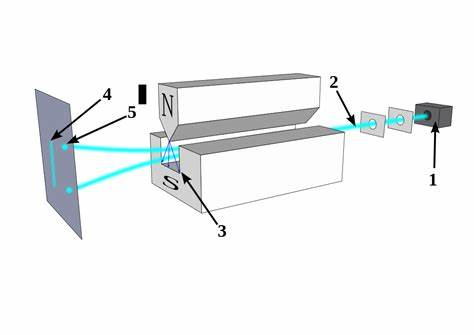
\includegraphics[width=0.75\textwidth]{fig/fig4-3.png}
  \label{fig:4-4}
  \caption{The setup of Stern-Gerlach experiment. (1) source; (2) hole; (3) inhomogeneous magnetic field; (4) the classical expectation and (5) the observation.}
\end{figure}

The corresponding force on the atom is
\begin{equation*}
  \mathbf{F} = \gamma \alpha \left( -S_x \hat{x} + S_z \hat{z} \right) .
\end{equation*}
However, as Eq.~\eqref{eq:4-113} suggested, due to the Larmor precession about $B_0$, $S_x$ oscillates rapidly and averages to zero.
The \textit{net} force is purely in the $z$ direction
\begin{equation}
  \label{eq:4-119}
 F_z = \gamma \alpha S_z
\end{equation}
and the beam is deflected up or down, in proportion to the $z$ component of the spin angular momentum.

In the more \textit{quantum} argument, we examine the process from the perspective of a reference frame that moves along with the beam.
In this frame the Hamiltonian starts out zero, turns on for a time $T$ and then turn off again
\begin{equation}
  \label{eq:4-120}
  H \left( t \right) =
  \begin{cases}
    0,~ ~ ~ &\text{for $t<0$} \\
    -\gamma \left( B_0 + \alpha a \right) S_z, ~ ~ ~ &\text{for $0\leq t \leq T$}\\
    0,~ ~ ~  &\text{for $t>T$}
  \end{cases},
\end{equation}
where we have ignore the $x$ component contribution from $\mathbf{B}$ for the same reason discussed before.
Suppose the atom has spin $\frac{1}{2}$ and starts out in the state
\begin{equation*}
\chi(t) = a \chi_+ + b \chi_- ~ ~ ~ \text{for $t\leq 0$}.
\end{equation*}
In the magnetic filed region where the non-zero Hamiltonian acts, we have
\begin{equation*}
\chi \left( t \right) = a \chi_+ e^{-i E_+ t/hbar} + b \chi_- e^{-iE_-t/\hbar} ~ ~ ~ \text{for $0\leq t \leq T$},
\end{equation*}
where
\begin{equation}
  \label{eq:4-121}
  E_{\pm} = \mp \gamma \left( B_0 +\alpha z \right) \frac{\hbar}{2}
\end{equation}
and hence it emerges in the state
\begin{equation}
  \label{eq:4-122}
  \chi \left( t \right) = \left( a e^{i\gamma T B_0/2} \chi_+ \right) e^{i \left( \alpha \gamma T/2 \right)z} + \left( b e^{-i\gamma T B_0/2} \chi_- \right) e^{-i \left( \alpha \gamma T/2 \right)z}.
\end{equation}
The two terms now carry \textit{momentum} in the $z$ direction
\begin{equation}
  \label{eq:4-123}
 p_z = \pm \frac{\alpha \gamma T \hbar}{2}.
\end{equation}
Thus $\chi_+$ will moves in the plus-$z$ direction and opposite for $\chi_-$ state.

\subsection{Addition of angular momenta}
Suppose now that we have two spin-$\frac{1}{2}$ particles---for example, the electron and the proton in the ground state of hydrogen.
Each can have spin up or spin down, so there are four possibilities in all\footnote{We consider the ground state, so there  will not any orbital angular momentum to worry about.}
\begin{equation}
  \label{eq:4-124}
 \ket{\uparrow \uparrow}, ~ \ket{\uparrow \downarrow},~ \ket{\downarrow \uparrow}, ~ \ket{\downarrow \downarrow},
\end{equation}
where the first arrow refer to the electron and the second to the proton.
We want to know what is the total angular momentum of the atom $\mathbf{S} \equiv \mathbf{S}_1 + \mathbf{S}_{2}$.
Since each of these four composite states in Eq.~\eqref{eq:4-124}, is an eigenstate of $S_z$, we have
\begin{equation*}
  S_z\ket{\chi_1 \chi_2} = \left( S_1 + S_2 \right) \ket{\chi_1 \chi_2} = \hbar \left( m_1 + m_2 \right) \ket{\chi_1 \chi_2}
\end{equation*}
So $m$ is just $m_1+m_2$:
\begin{align*}
  m &=1 ~ ~ ~ \ket{\uparrow \uparrow}\\
  m &=0 ~ ~ ~ \ket{\uparrow \downarrow}\\
  m &=0 ~ ~ ~ \ket{\downarrow \uparrow}\\
  m &=-1 ~ ~ ~ \ket{\downarrow \downarrow}.
\end{align*}

At first glance, this does not look right: $m$ is suppose to advance in integer steps from $-s$ to $+s$ where $s=1$ in our case.
However, there is an ``extra'' state with $m=0$.
One way to untangle this problem is to apply the lowering operator to the state $\ket{\uparrow \uparrow}$
\begin{equation*}
  S_- \ket{\uparrow \uparrow} = \hbar \left( \ket{\downarrow \uparrow} + \ket{\uparrow \downarrow} \right).
\end{equation*}
Evidently, in the notation of $\ket{sm}$, the three stats with $s=1$ are
\begin{equation}
  \label{eq:4-125}
  s = 1 ~ \text{(triplet state)} ~ \to
  \begin{cases}
    \ket{11} &= \ket{\uparrow \uparrow} \\
    \ket{10} &= \frac{1}{\sqrt{2}} \left( \ket{\uparrow \downarrow} + \ket{\downarrow \uparrow} \right)\\
    \ket{1-1} &= \ket{\downarrow \downarrow}
  \end{cases}.
\end{equation}
This is called the \textbf{triplet} combination.
Meanwhile, the orthogonal state with $m=0$ carries $s=0$
\begin{equation}
  \label{eq:4-126}
  s = 0 ~ \text{(singlet state)} ~ \to \ket{00} = \frac{1}{\sqrt{2}} \left( \ket{\uparrow\downarrow} - \ket{\downarrow \uparrow} \right).
\end{equation}

We found that the combination of two spin-$\frac{1}{2}$ particles can carry a total spin of $1$ and $0$, depending on whether they occupy the triplet or the single configuration.
To verify this, we will prove that the triplet states are eigenvectors of $S^2$ with eigenvalue $\hbar^{2} s \left( s+1 \right) = 2\hbar^{2}$ and single is for eigenvalue $0$.
Now,
\begin{equation}
  \label{eq:4-127}
 S^2 = \left( \mathbf{S}_1 + \mathbf{S}_2 \right) \cdot \left( \mathbf{S}_1 + \mathbf{S}_2 \right) = S_1^2 + S_2^2 + 2 \mathbf{S}_1 \cdot \mathbf{S}_2.
\end{equation}
Using Eq.~\eqref{eq:4-102} and Eq.~\eqref{eq:4-104}, we have
\begin{align*}
  & \mathbf{S}_1 \cdot \mathbf{S}_2 \ket{\uparrow \downarrow} \\
  =& \left( S_{x1}S_{x2} + S_{y1}S_{y2} + S_{z1}S_{z2} \right) \ket{\uparrow\downarrow}\\
  =& \frac{\hbar^{2}}{4} \left( 2\ket{\downarrow\uparrow} - \ket{\uparrow\downarrow} \right).
\end{align*}
Similarly,
\begin{equation*}
   \mathbf{S}_1 \cdot \mathbf{S}_2 \ket{\downarrow \uparrow}  =  \frac{\hbar^{2}}{4} \left( 2 \ket{\uparrow \downarrow} - \ket{\downarrow\uparrow} \right).
\end{equation*}
Then returning to Eq.~\eqref{eq:4-125}, we have
\begin{equation}
  \label{eq:4-128}
  S^2 \ket{10} = \left( \frac{3\hbar^{2}}{4} + \frac{3\hbar^{2}}{4} + 2 \frac{\hbar^{2}}{4} \right) \ket{10} = 2\hbar^2 \ket{10},
\end{equation}
so $\ket{10}$ is indeed an eigenstate of $s^2$ with eigenvalue $2\hbar^{2}$.
We can did the similar calculation for $\ket{00}$ and we have $S^2 \ket{00}= 0 \ket{00}$.

This is the simplest example of a larger problem: If you combine spin $s_1$ with spin $s_2$, the total spins $s$ you can get is
\begin{equation}
  \label{eq:4-129}
 s = \left( s_1 + s_2 \right), \left( s_1+s_2-1 \right), \ldots, \abs{s_1-s_2},
\end{equation}
where they are in integer steps.
For example, if you package together a particle of spin $\frac{3}{2}$ with a particle of spin $2$, you could get a total spin of $\frac{7}{2}$, $\frac{5}{2}$, $\frac{3}{2}$, or $\frac{1}{2}$, depending on the configuration.
Another example, if a hydrogen atom is in the state $\psi_{nlm}$, the net angular momentum of the electron is $l+ \frac{1}{2}$ or $l - \frac{1}{2}$;
if you now throw in a \textit{proton}, the atom's total angular momentum quantum number is $l+1$, $l$, or $l-1$.

The combined state $\ket{sm}$ with total spin $s$ ans $z$-component $m$ will be some linear combination of the composite states $\ket{s_1 m_1}\ket{s_2 m_2}$:
\begin{equation}
  \label{eq:4-130}
 \ket{sm}  = \sum_{m_1+m_2=m} C_{m_1m_2m}^{s_1s_2s} \ket{s_1 m_1} \ket{s_2 m_2}.
\end{equation}
The constants $C_{m_1m_2m}^{s_1s_2s}$ are called \textbf{Clebsch-Gordan coefficients}
The simplest case are listed in Fig.~\ref{fig:4-5}.
\begin{figure}[t]
  \centering
  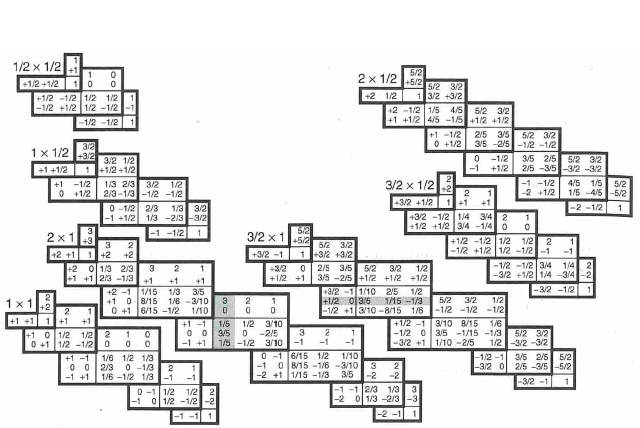
\includegraphics[width=0.95\textwidth]{fig/fig4-4.png}
  \label{fig:4-5}
  \caption{Clebsch-Gordan coefficients. A square root sign is understood for every entry; the minus sign, if present, goes outside the radical.}
\end{figure}
For example, the shaded column of $2\times 1$ table tell us that
\begin{equation*}
\ket{30} = \frac{1}{\sqrt{5}}\ket{21}\ket{1-1} + \sqrt{\frac{3}{5}}\ket{20}\ket{10} + \frac{1}{\sqrt{5}}\ket{2-1}\ket{11}.
\end{equation*}
In particular, if two particles (of spin $2$ and spin $1$) are at rest in a box, and the total spin is $3$, and its $z$ component is $0$ (where $\ket{30}$), then a measurement of $S_z^1$ could return the value $\hbar$ (with probability $\frac{1}{5}$), or $0$ (with probability $\frac{3}{5}$), or $-\hbar$ (with probability $\frac{1}{5}$).

These tables also work the other way around
\begin{equation}
  \label{eq:4-131}
 \ket{s_1 m_1} \ket{s_2 m_2} = \sum_s C_{m_1m_2m}^{s_1s_2s} \ket{sm}.
\end{equation}
For example, the shaded row in the $\frac{3}{2}\times 1$ table tells us that
\begin{equation*}
  \ket{\frac{3}{2} \frac{1}{2}} \ket{10} = \sqrt{\frac{3}{5}} \ket{\frac{5}{2} \frac{1}{2}} + \sqrt{\frac{1}{15}} \ket{\frac{3}{2} \frac{1}{2}} - \sqrt{\frac{1}{3}} \ket{\frac{1}{2} \frac{1}{2}}
\end{equation*}
If you put particles of spin $\frac{3}{2}$ and spin $1$ in the box, and you know that the first has $m_1= \frac{1}{2}$ and the second has $m_2=0$, and you measure the total spin, $s$, you could get $\frac{5}{2}$ (with probability $\frac{3}{5}$), or $\frac{3}{2}$ (with probability $\frac{1}{15}$), or $\frac{1}{2}$ (with probability $\frac{1}{3}$).

In a mathematical sense this is all applied \textbf{group theory}---what we are talking about is the decomposition of the direct product of two irreducible representations of the rotation group into a direct sum of irreducible representations.










%%% Local Variables:
%%% mode: latex
%%% TeX-master: "main"
%%% End:
